\documentclass[11pt,twoside,a4paper]{article}
\usepackage{amsmath}
\usepackage{graphicx}
\usepackage{rotating}
\usepackage{tikz}
\usepackage[backend=bibtex]{biblatex}
%\usepackage{natbib}
\begin{document}

\title{Comparison of primary glioblastoma Single-cell and Tissue RNA-seq co-expression networks}
\author{Brian Arand \and Raghu Machiraju \and Kun Huang}
\maketitle

\begin{abstract}
Hello World! 
\end{abstract}

\section{Introduction}
The isolation of individual cells’ transcriptome profiles has been largely a theoretical concept to bioinformaticians. And accordingly, transcriptomic inquiry has been limited to those questions regarding tissues— potentially composed of a heterogeneous hodgepodge of cellular types, subtypes, and states. But with the advent of Single-Cell RNA sequencing (RNASeq) technology, comes the potential for refined resolu-tion in transcriptomic datasets. And expectedly, recent publications suggest a peaking interest in this new landscape of informatics. It has been shown that many bioinformatics techniques that were developed for population-cell tissue samples can be effectively applied to single-cellular datasets. However, co-expression network analysis has largely been an unexplored area of analysis in regards to single-cell RNASeq data. To fill this gap, we leverage this new technology to construct and analyze gene co-expression networks for primary glioblastoma single-cell samples. Glioblastoma is widely known to be a heterogeneous cancer, making it a prime candidate for single-cellular inquiries. For instance, it is hypothesized that the averaging of single-cells’ profiles within a tissue sample may mask or otherwise confound downstream gene correlations based analysis.  Correlation between two genes may exist across tissue samples purely due to changing proportion of cellular subtypes within those samples. However, a single-cellular perspective, of the same tumors may theoretically filter out those artificial tissue-level correlations. And so correlation based analysis, like co-expression network analysis, require study. In our work, we begin this journey by looking at network mining, module detection, and gene enrichment analysis at both the single-cell and population of cell (tissue sample) levels. The final goal of this work is to shed light on the convoluted intricacies of inter-cellular genomic landscape of glioblastoma tissue from a single-cellular perspective.

\section{Method}

\begin{figure}[t]
\centering
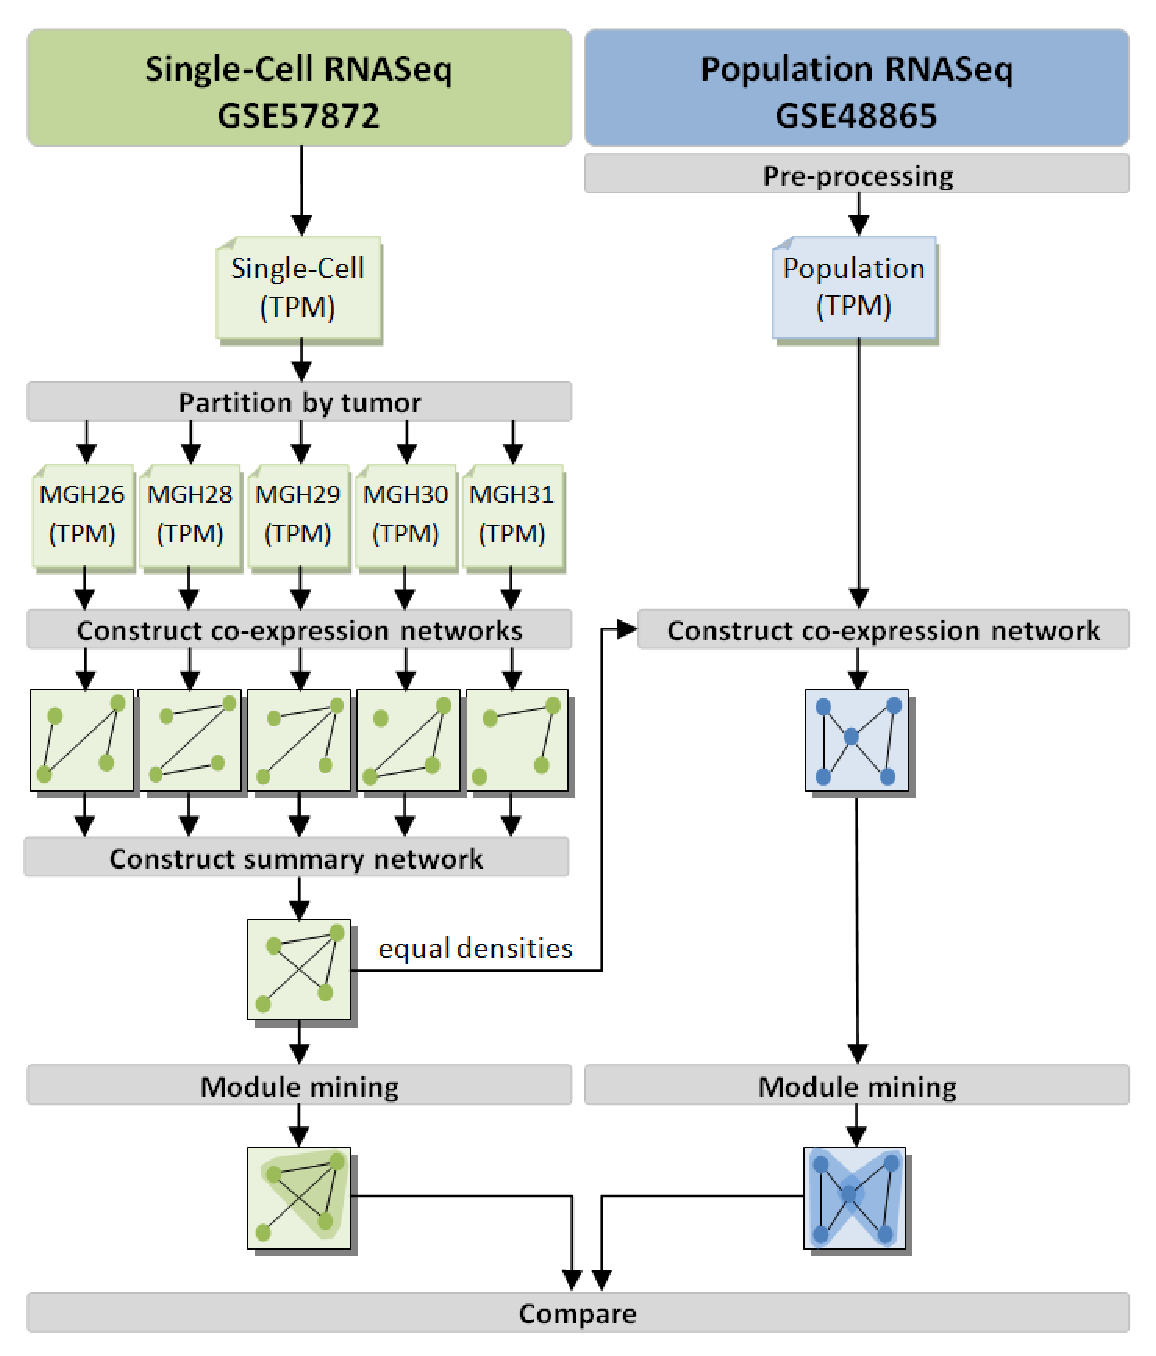
\includegraphics[width=80mm]{Figures/Workflow}
\caption{Workflow}
\label{Workflow Figure}
\end{figure}

We analyzed two glioma datasets: GSE57872, the data presented in Single-cell RNA-seq highlights intratumoral heterogeneity in primary glioblastoma \cite{Patel}, and GSE48865, the data presented in RNA-seq of 272 gliomas revealed a novel, recurrent PTPRZ1-MET fusion transcript in secondary glioblastomas \cite{Bao}. GSE57872 consists of single-cell samples whereas GSE48865 consists of more-traditional, population-of-cell (or tissue) samples. After preprocessing each dataset independently (steps explained in following sections), we step each dataset through a coexpression-network analysis workflow. This workflow has a number of parts: correlation calculation, network construction, module detection, and enrichment analysis. Necessary variations to this workflow per dataset are explained in sections to follow. 

\subsection{Single-Cell RNASeq Samples }

We analyzed GSE57872: the data presented by Patel et al. in Single-cell RNA-seq highlights intratumoral heterogeneity in primary glioblastoma (Patel, et al., 2014). This data is comprised of normalized gene expression values for 5,948 genes for 430 single-cell samples selected by flow cytometry cell sorting and micromanipulation from 5 different primary glioblastomas labeled: MGH26, MGH28, MGH29, MGH30, and MGH31. The cells were then sequenced using SMARTseq protocol (Ramskold, et al., 2012). Alignment to hg19 was performed with Bowtie (version 1.1.1) (Langmead, Trapnell, Pop, \& Salzberg, 2009) and the authors calculated TPM (transcripts per million) values using RSEM (version 1.2.3) (Li \& Dewey, 2011).The final reported values were log-transformed and mean-shifted per gene. More formally, let xsi be the TPM enrichment value for the ith gene of sample s. And let Nt be the sample size of tumor t, then the analogous, final reported value, ysi , would be: 
\begin{figure}[t]
\centering
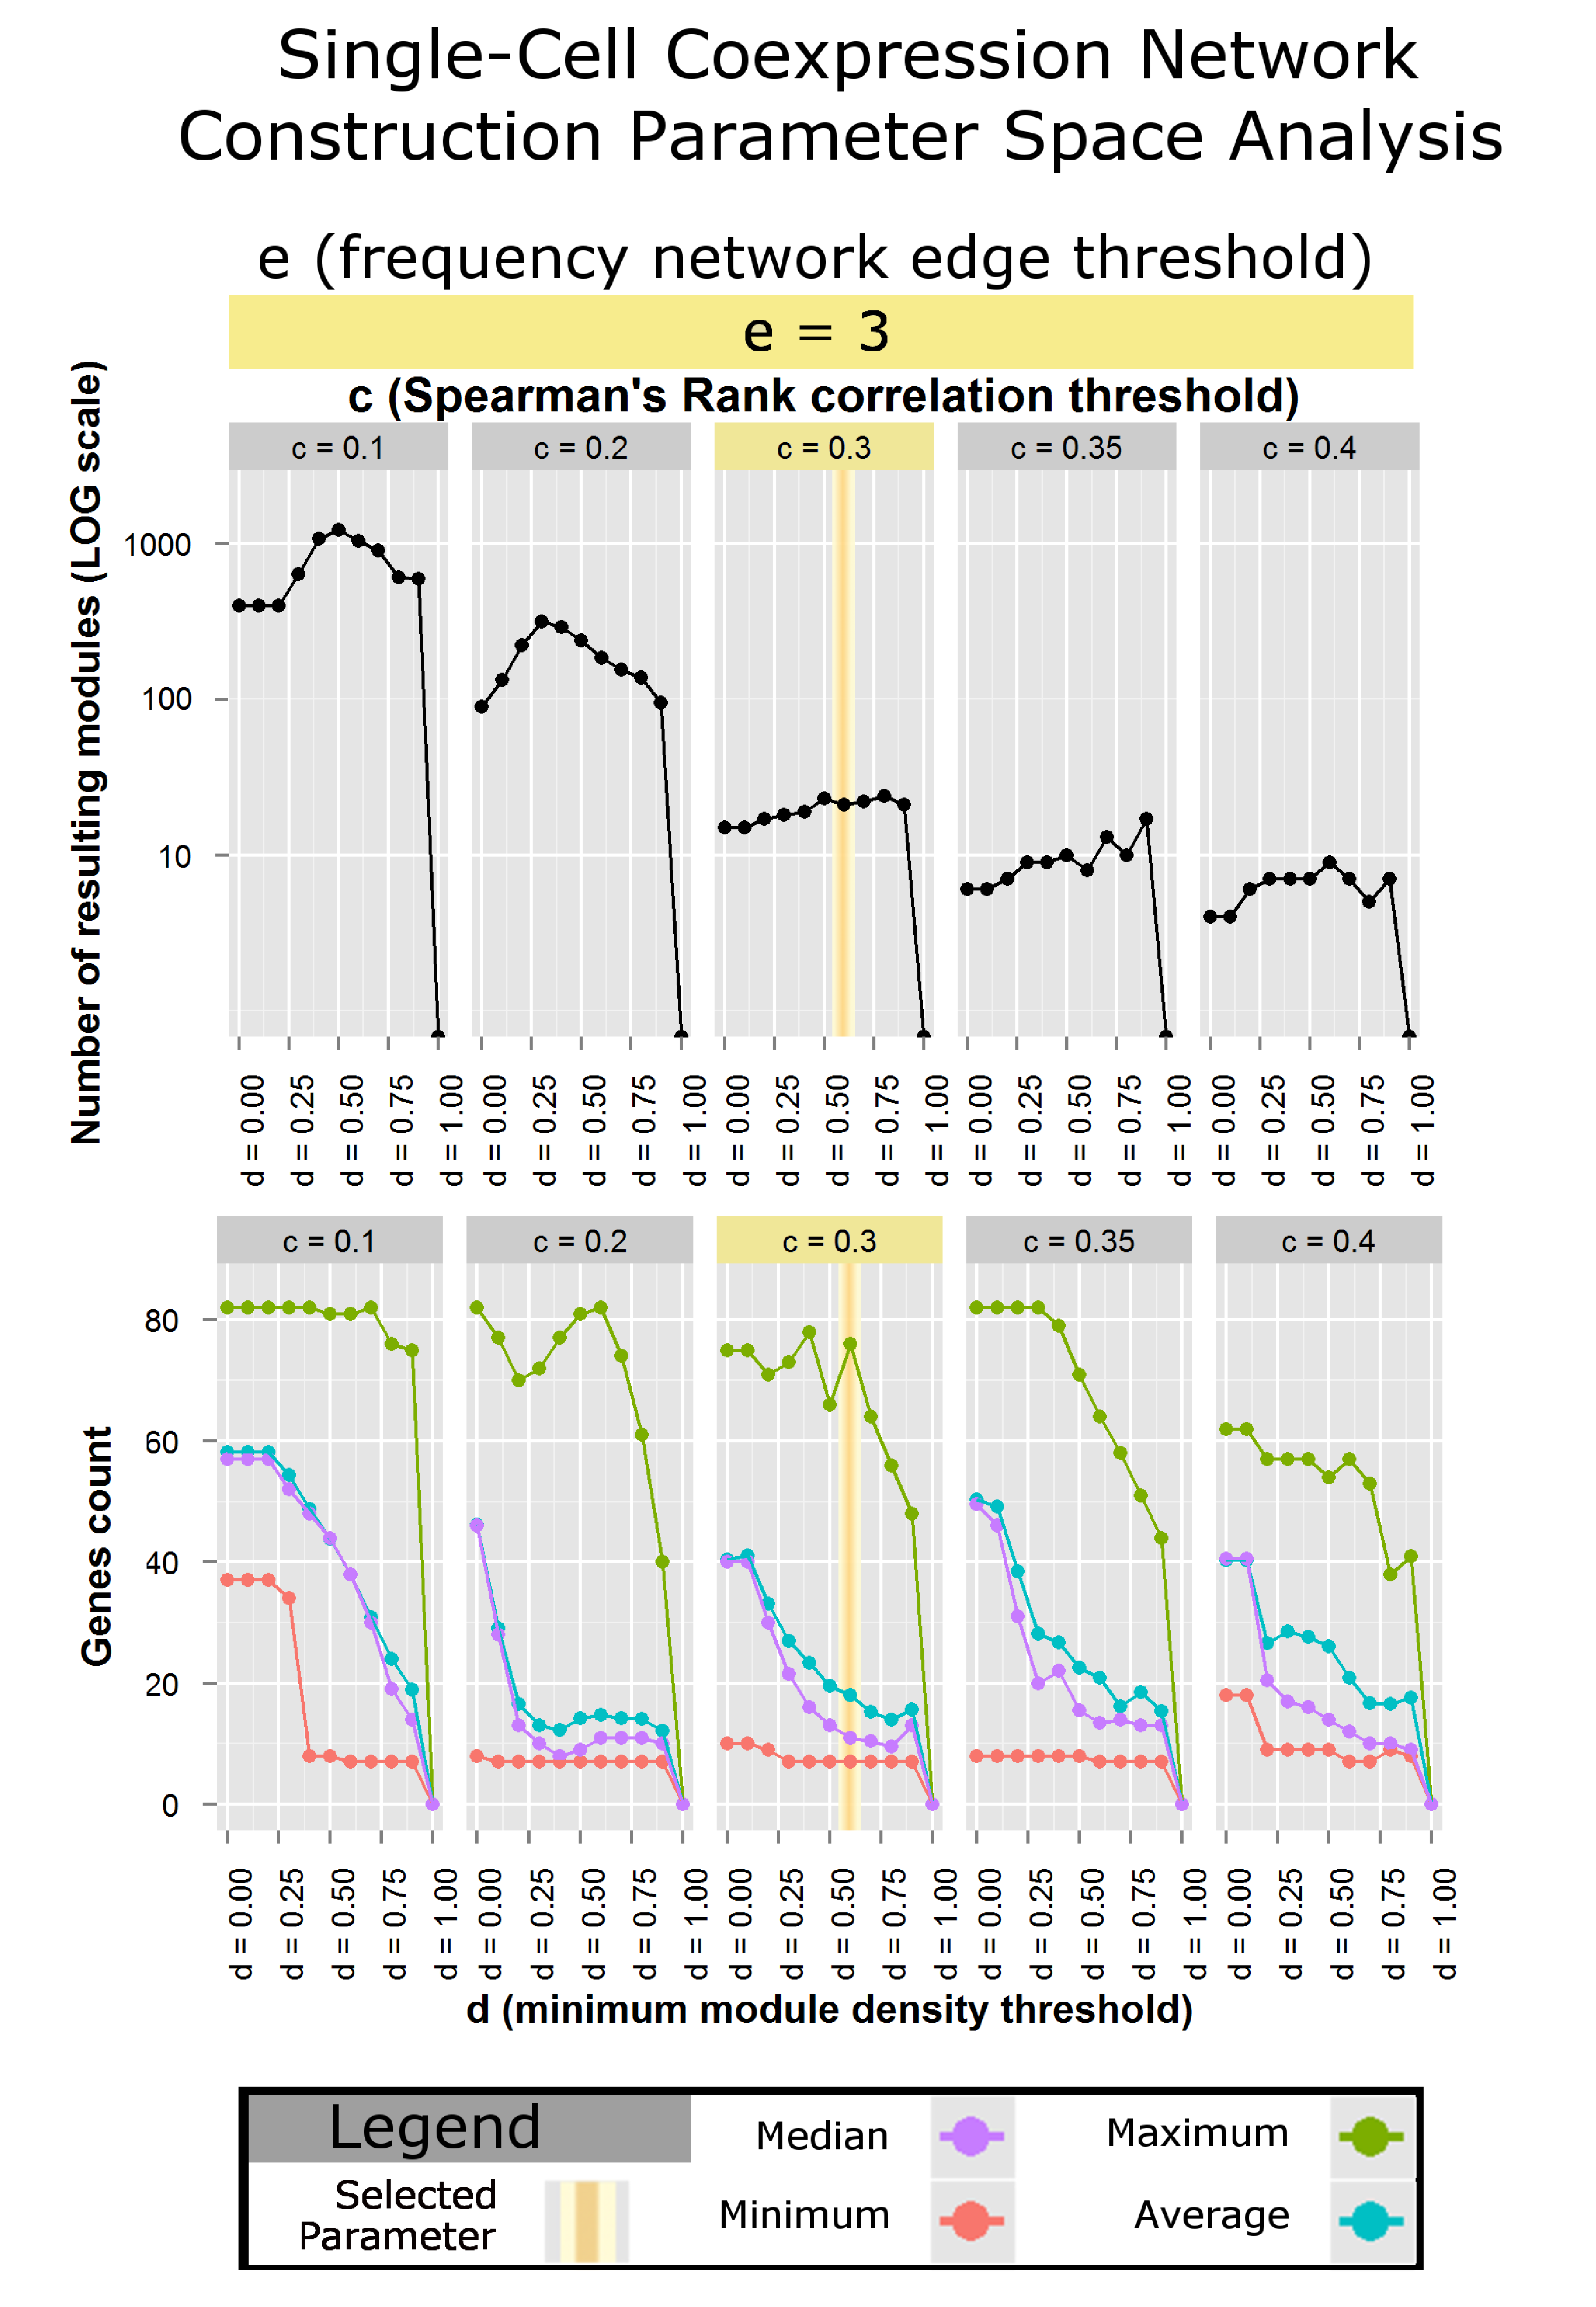
\includegraphics[width=80mm]{Figures/ParameterSpaceE=3}
\caption{Parameterization space analysis.}
\label{Parameter Space Figure}
\end{figure}

\begin{equation}\label{equation1}
\frac{\sum_{s} \log_2(x_{si} + 1)} {N_t}
\end{equation}

\begin{equation}\label{equation2}
\sum_{s} \log_2(x_{si} + 1)-y_i
\end{equation}

\subsubsection{Network Construction}
In our analysis, single-cell samples were grouped by tumor of origin, $t$. For each group, a gene-by-gene Spearman’s rank correlation matrix was calculated: 

\begin{equation}\label{equation3}
 P_t = \left[ \begin{array}{ccc}
\rho_{11t} & \ldots & \rho_{1kt} \\
\vdots & \ddots & \vdots \\
\rho_{k1t} & \ldots & \rho_{kkt}i \end{array} \right]
\end{equation}%

Where $\rho_{ijt}$ is the Spearman’s correlation between the $i^{th}$ and $j^{th}$ gene of tumor $t$. Co-expression matrices were then created by filtering at the same Spearman’s rank threshold, $c$, to produce binary matrices, $B_t$, per tumor. 

\begin{equation}\label{equation4}
B_t = \left[ \begin{array}{ccc}
b_{11t} & \ldots & b_{1kt} \\
\vdots & \ddots & \vdots \\
b_{k1t} & \ldots & b_{kkt}i \end{array} \right] \\
, b_{ijt}=\{ \begin{array} {cc}
1, & \vert\rho_{ijt}\vert\ge c \\
0, & o.w. \\
\end{array}
\end{equation}

This is analogous to cutting a co-expression network at a given edge threshold. After analyzing the distribution of resulting networks’ densities (Figure 1.a) we settled on a threshold of 0.3 with an associated frequency network density of (0.04). We point out that this threshold is low, but we argue that it is a necessary trade-off given the distribution of correlations (Figure 1.b). It is expected to see such non-concordant data, because current single-cell RNASeq technology is known to produce noisy data (need a reference for this).

The binary matrices were then aggregated into a single frequency matrix, F. This aggregation is performed in an attempt to attenuate patient-specific signals and focus, rather, on glioblastoma-specific patterns of gene co-expression.

\begin{equation}\label{equation5}
F = \left[ \begin{array}{ccc}
\sum_{t}b_{11t} & \ldots & \sum_{t}b_{1kt} \\
\vdots & \ddots & \vdots \\
\sum_{t}b_{k1t} & \ldots & \sum_{t}b_{kkt} \end{array} \right]
\end{equation}

\subsubsection{Module Detection}
This frequency matrix was then fed into the CODENSE software to be converted into a summary network, $S$, and then mined for high-density modules (Hu, Yan, Huang, Han, \& Zhou, 2005).  

\begin{equation}\label{equation6}
X=(V,E), where v_i,v_j \in V and (v_i,v_j) \in E \leftrightarrow f_ij \ge e
\end{equation}

CODENSE then reported the modules that meet some minimum density threshold, d. At the suggestion of the CODENSE authors and after analyzing the effect perturb-ing d has on the number and size of the resulting modules, we chose a minimum den-sity threshold of 0.6. We wanted to maximize our parameter d to ensure dense mod-ules to ensure their biological significant. Note that in figure 2, heightened values of d can produce can drastically affect the output number and size of modules. Our selection of d = 0.6 marks the upper limit of where this non-robust behavior starts in our selected parameter space sampling resolution. At the selected parameterization CODENSE reported 21 dense, first-order modules. These relatively high thresholds will guarantee that our resulting modules will be dense and highly representative of tumors as a whole rather than dominated by signal from just a single tumor of origin (see Figure 2).  We find that these are necessary steps in order to extract meaningful co-expression from data that is relatively noisy and will so few tumors of origin to work with.

\subsection{Population Tissue Samples}
Our population-tissue control comes from GEO accession GSE48865. 274 glioma tissue samples make up this dataset, of which, 59 were identified as primary, stage-4 glioblastoma tissue samples. We filtered out any reads from the 59 samples with more than 10\% of its nucleotides designated as unknown bases, and any read with more than 50\% of its bases having Sanger phred+33 quality scores less than 5. After filtering, we retained 1,388,064,773 reads in total. 

Each filtered sample was then aligned to hg19 transcriptome (GRCh37) using bow-tie (version 1.1.1 with default parameters provided by RSEM) and TPM values per gene were estimated using RSEM (version 1.2.3). 73\% of the reads were aligned successfully either uniquely or multi-mapped. 

TPM values were adjusted again as in equation (2). Genes were then filtered to retain only those that were highly expressed across the 59 samples. The $i^{th}$ gene was filtered out if $y_{i} <= 4.5$. We retained 6,932 genes after filtering.
\subsubsection{Network Construction}

Spearman’s Rank correlation was calculated for all genes pair-wise. No further network aggregation step was required for this data set. 

\subsubsection{Module Detection}

Quasi-Clique Merger (eQCM) (Xiang Y FAU Xiang, Zhang CQ FAU Zhang, \& Huang K FAU Huang) was employed to mine the modules in the population sample network with parameters:

\subsection{Enrichment}

Module sets derived from both the single-cell network and population tissue sam-ple network were then ontology enriched. Modules were enriched for all terms in Gene Ontology Consortium’s biological process (BP), cellular component (CC), and molecular function (MF) human ontologies using the David Bioinformatics Resources (version 6.7) Functional Annotation Tool (Huang DW FAU Huang, Sherman BT FAU Sherman, \& Lempicki RA FAU Lempicki) (Huang DW FAU Huang, Sherman BT FAU Sherman, \& Lempicki RA FAU Lempicki).

\section{Results}
\subsection{Single-Cell Module Enrichment}

\begin{figure}[t]
\centering
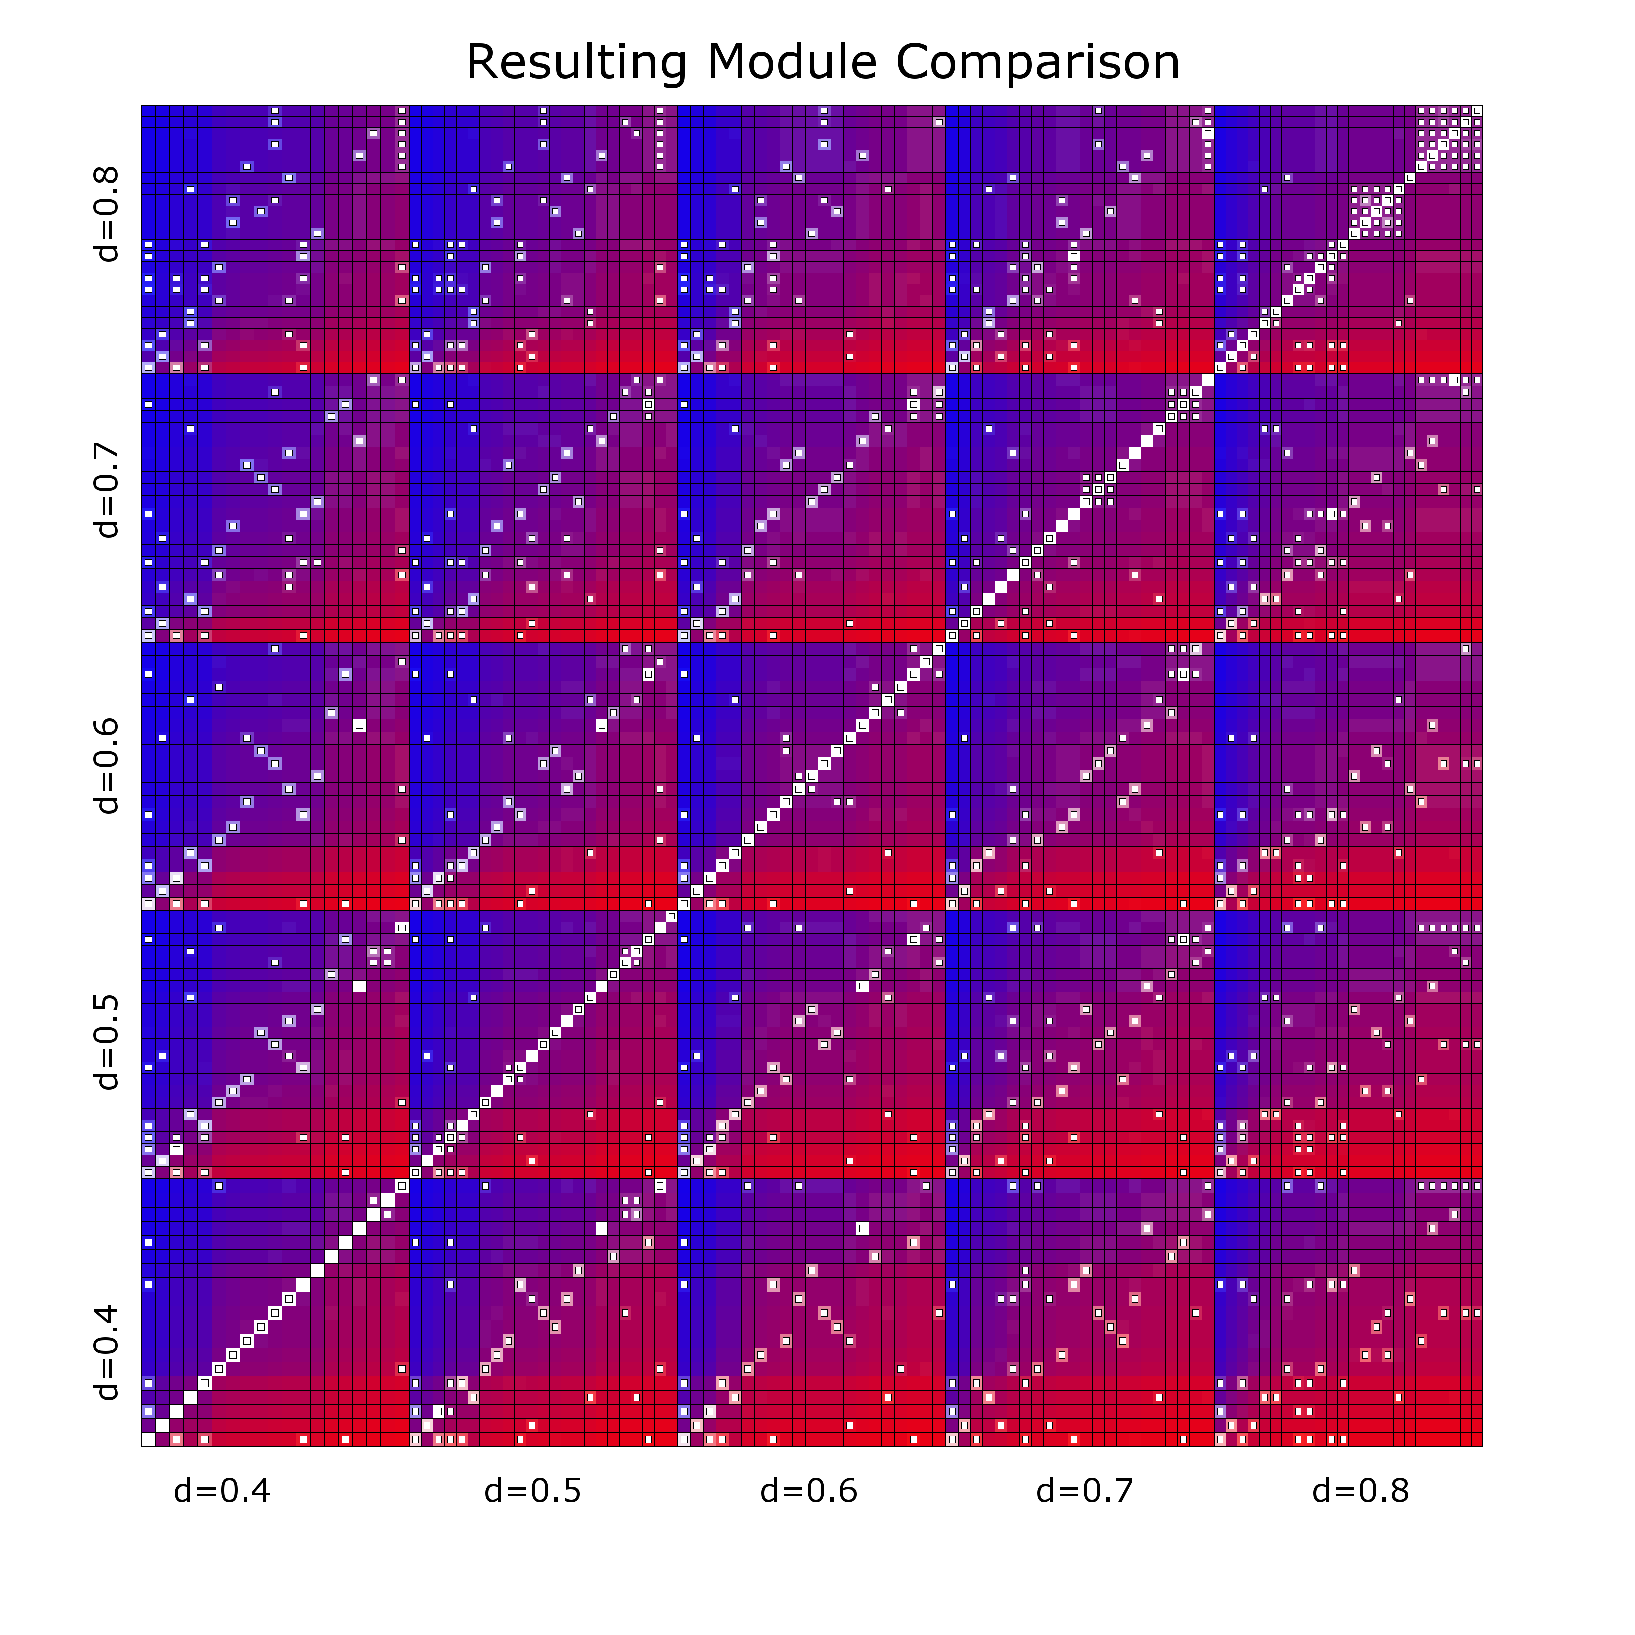
\includegraphics[width=100mm]{Figures/moduleStaryNight}
\caption{Output module co-enrichment Starry Map diagram.}
\label{Starry Map Figure}
\end{figure}

\subsection{Population Module Enrichment}

\begin{sidewaysfigure}
	\centering
	
\begin{tikzpicture}[scale=4]
        \fill[blue] (0,0) rectangle(2,1.5);  
    \end{tikzpicture}
	\caption{Parameterization space analysis.}
	\label{Parameter Space Figure}
\end{sidewaysfigure}

Something something update...

\section{Discussion}
Compare with Yang paper
Cell cycle and extra cellular matrix ontologies are less 

Caveats:
	Not many tumors in study and thereby not many original networks before aggregation into frequency network.
\section{Conclusion}
\section{References}

\end{document}
